\documentclass[10pt]{beamer}

\batchmode

%导入一些用到的宏包
\usepackage{graphicx}
\usepackage{animate}
\usepackage{url}
\usepackage{ulem}

\usepackage{xeCJK} %导入中文包
\setCJKmainfont{SimHei} %中文字体采用黑体  Microsoft YaHei

\usetheme{metropolis}
\usepackage{appendixnumberbeamer}

\usepackage{booktabs}
\usepackage[scale=2]{ccicons}

\usepackage{pgfplots}
\usepgfplotslibrary{dateplot}

\usepackage{xspace}
\newcommand{\themename}{\alert{\textsc{metropolis}}\xspace}

\title{Distributed Hash Table: Fair and Free}
\subtitle{PPCA 2021\ 大作业\ 分布式哈希表}
\date{\today}
\author{林超凡}
\institute{ACM Class 2020}

\begin{document}
\maketitle

%0. 目录页
\begin{frame}{Contents}
	\addtocounter{framenumber}{-2}
	\thispagestyle{empty}
	\tableofcontents
	\end{frame}
\end{frame}

%1. Intro
\section{Introduction}

\begin{frame}[fragile]{客户端/服务器 与 P2P网络}
  \begin{itemize}
  \item C/S架构
  \item 对等网络(Peer to Peer Networking)
\end{itemize}

\centering
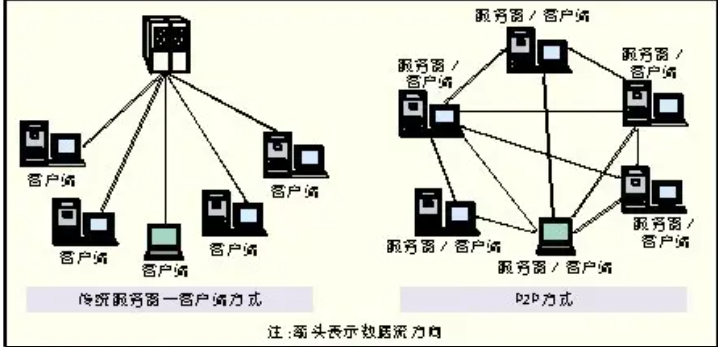
\includegraphics[scale=0.6]{figure/p2p.png}

\end{frame}

\begin{frame}[fragile]{RPC}
  RPC是什么? Remote Procedure Call
  一个客户端想要调用另一个客户端的方法

\\[20pt]

\begin{figure}
\centering
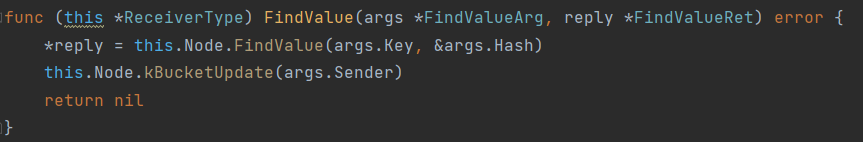
\includegraphics[scale=0.6]{figure/code1.png}
\end{figure}

\\[20pt]

流程 (假设A想调用B的方法): 
\begin{itemize}
\item	A.Diag(B.ip)
\item 	A.Call(方法名, 参数, 返回地址)...
\item  B收到Call, 执行对应方法
\end{itemize}}

\end{frame}

\begin{frame}[fragile]{可能遇到的问题}

也许...
	\begin{itemize}
		\item 某一客户端电源线被踢掉 (ForceQuit)
		\item 网络通信繁忙
		\item 恶意的网络攻击
	\end{itemize}

\end{frame}

%2. Chord
\section{Chord Protocol}
\begin{frame}{最朴素的分布式想法}

每个客户端采用同样的哈希函数: 一致性哈希 (比如SHA-1)
\\[20pt]
每个客户端维护一部分数据——分块
\\[20pt]
接入网络时候,原有客户端将一部分数据转移给新节点;
退出网络时,将自己的数据转移给其它节点.

\end{frame}

\begin{frame}{最朴素的分布式想法}

\alert{A:} \{data1, data2, data3\}

\end{frame}

\begin{frame}{最朴素的分布式想法}

\alert{A:} \{data1, data2\}

\alert{B:} \{data3\}

\end{frame}

\begin{frame}{最朴素的分布式想法}

\alert{A:} \{data1\}

\alert{B:} \{data3\}

\alert{C:} \{data2\}

\end{frame}


\begin{frame}{最朴素的分布式想法}

\alert{B:} \{data1, data3\}

\alert{C:} \{data2\}

\end{frame}

\begin{frame}{改进}

规定一些客户端间共同遵守的规则, 我们称为\alert{协议(protocol)}
	\begin{itemize}
		\item 哪些数据归谁管?
		\item 怎样快速地查找数据?
		\item 节点强制退出怎样做到尽量不丢失数据?
	\end{itemize}
在哈希表中,我们可以将数据简单地视为 Key-Value 对研究\\
同时每个客户端我们下面称作一个节点(Node)
\end{frame}

\begin{frame}{Chord环}

任何哈希函数都有它的值域。对于SHA-1, $[0, 2^{160})$ \\
能否给每个节点也分配一个哈希值?\alert{hash=SHA1(IP)}

\begin{figure}
\centering
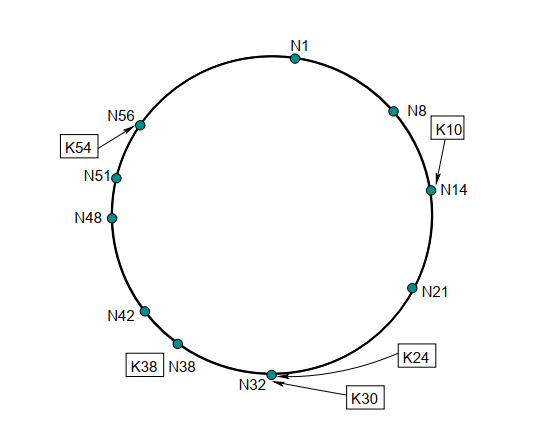
\includegraphics[scale=0.5]{figure/ring.png}
\end{figure}

这样数据对和节点都有哈希值(称作id, identifier)\\
节点将环分成好几段,规定每个节点维护自己上面(逆时针走)那段值域的数据

\end{frame}

\begin{frame}{高效地查找:Finger Table}
每个节点都有唯一的前驱(predecessor)、后继(successor)

\begin{figure}
\centering
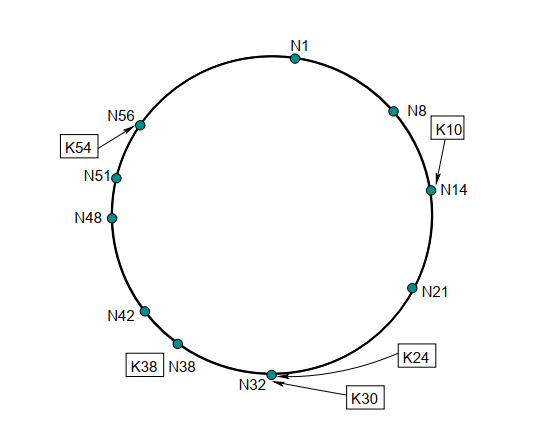
\includegraphics[scale=0.5]{figure/ring.png}
\end{figure}

\\[20pt]

查找: 对于给定的key值, 找到其后面第一个节点,即 \alert{findSuccessor}
\end{frame}

\begin{frame}{高效地查找:Finger Table}
不止于维护后继: \alert{Finger Table}

对于每个点(哈希值为id),维护 $id+1, id+2, \dots, id+2^M$ 的后继Node

\begin{figure}
\centering
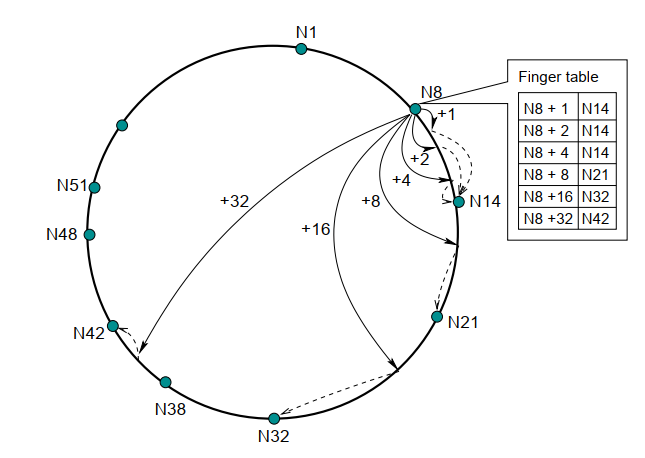
\includegraphics[scale=0.5]{figure/finger.png}
\end{figure}

\\[20pt]

\end{frame}

\begin{frame}{高效地查找:Finger Table}

\alert{n.findSuccessor(key):} \ $\ \log N$ \\
\begin{itemize}
\item
如果 key 值在自己与后继之间,返回后继 \\
\item
否则,给 finger 表里离 key 值最近的且为其前继的节点发送 findSuccessor RPC \\
\item
n'.findSuccessor
\end{itemize}


\begin{figure}
\centering
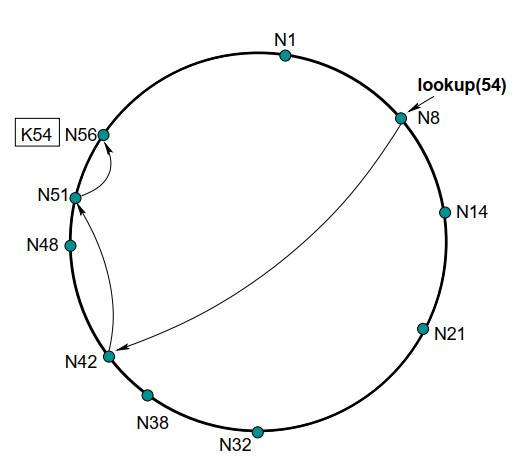
\includegraphics[scale=0.5]{figure/lookup.png}
\end{figure}

\\[20pt]

\end{frame}

%3. 实现细节
\section{Implementation}
\begin{frame}{Golang}
C < go < C++

\\[20pt]

\begin{itemize}
\item 为并发而生 go routinue
\item 简洁且与C高度相似的语法
\item 零值初始化以及自动内存回收

\end{itemize}
\end{frame}

\begin{frame}{Golang}
虽然...

\begin{figure}
\centering
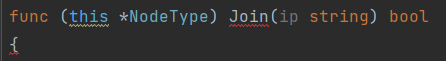
\includegraphics[scale=0.9]{figure/code2.png}
\end{figure}

\\[20pt]

\end{frame}

\begin{frame}{接口需求}

\begin{figure}
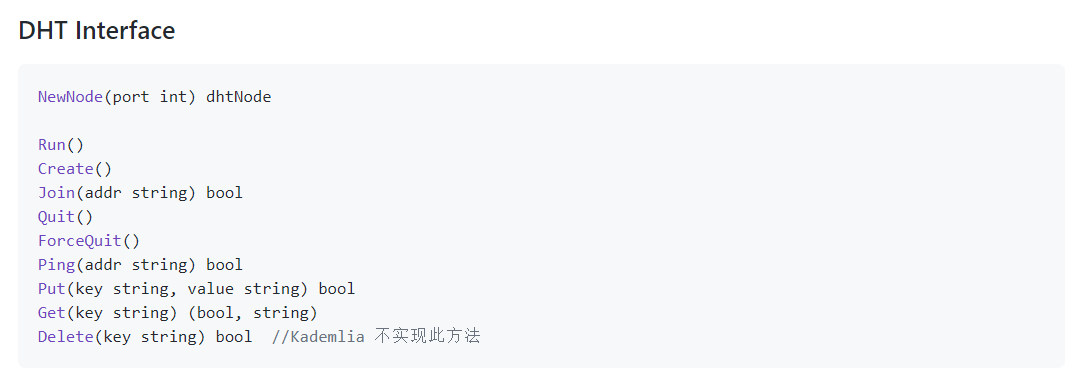
\includegraphics[scale=0.9]{figure/interface.png}
\end{figure}

\\[20pt]

\end{frame}

\begin{frame}{设计思路}

\alert{PubNode:} 实现目标 interface \\

\\[20pt]

\alert{Receiver:} 实现rpc服务 \\

\\[20pt]

\alert{Node:} 实现chord协议中的节点 \\

\\[20pt]

\end{frame}

\begin{frame}{设计思路}

rpc设计相关...

\begin{itemize}
\item 使用 go 的 net 包, 每个节点开一个 Server 和 Client
\item 使用 net 包中的 Diag/Call 实现 rpc \\
	   * 为防止因网络繁忙而阻塞,每次呼叫3次
\item 将需要远程调用的方法封装为rpc Methods
\end{itemize}

\begin{figure}
\centering
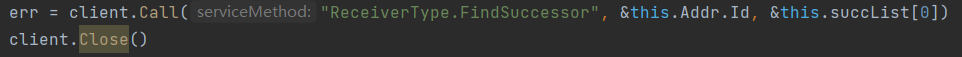
\includegraphics[scale=0.5]{figure/code3.png}
\end{figure}

\end{frame}

\begin{frame}{设计思路}

Node设计相关...

\begin{itemize}
\item \alert{FixFinger} 单开线程并行维护,每次修复一位,然后将位置加 1 准备对下个位置 Fix
\item \alert{FindSuccessor} 按照论文编写,跳 Finger 表,且要求 Ping 的通,若 Finger 表全部失效则访问后继
\item \alert{ForceQuit} 每个节点备份自己后继的数据,同时维护后继列表,当维护后继列表过程中发现后继失效,将备份数据合并到后继列表第一个有效节点。
\end{itemize}

\end{frame}

\begin{frame}{遇到的问题}

并行中的\alert{死锁}问题: github.com/sasha-s/go-deadlock

\\[20pt]

因为维护周期导致的\alert{Wrong Answer}: 缩短维护周期

\\[20pt]

环境导致的\alert{socket:too many open files}等问题: 使用虚拟机, 修改ulimits和config

\end{frame}

\begin{frame}{开发周期}

\begin{figure}
\centering
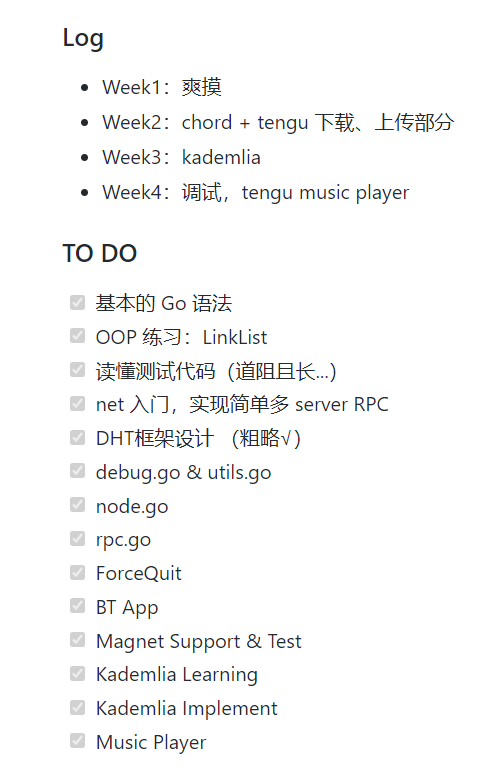
\includegraphics[scale=0.5]{figure/log.png}
\end{figure}

\end{frame}

\begin{frame}{一个测试工程师走进一个酒吧...}

\begin{figure}
\centering
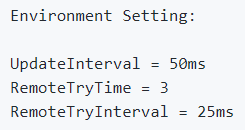
\includegraphics[scale=0.8]{figure/env.png}
\end{figure}

\\[20pt]

\begin{figure}
\centering
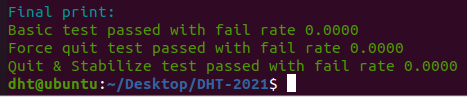
\includegraphics[scale=0.6]{figure/performance.png}
\end{figure}

\end{frame}

%4. Kad 和 Tengu 介绍
\section{Kademlia \& Tengu}

\begin{frame}{Kademlia Protocol}

\alert{Chord 中的距离:} $dis(a,b) = (a - b + 2^{160}) \mod 2^{160}$ \\

\\[20pt]

\alert{Kademlia 中的距离:} $dis(a,b) = a \otimes b$ \\

\end{frame}

\begin{frame}{Kademlia Protocol}

\url{https://zhuanlan.zhihu.com/p/38425656}

\begin{figure}
\centering
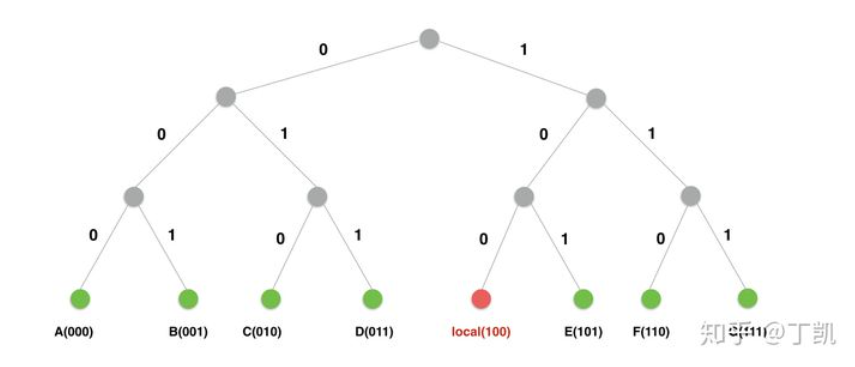
\includegraphics[scale=0.6]{figure/kad.png}
\end{figure}

\end{frame}

\begin{frame}{Tengu}

是一个支持上传/下载的文件分享系统 \\ 
\sout{也可以用来在PPCA摸鱼时听歌}

\begin{figure}
\centering
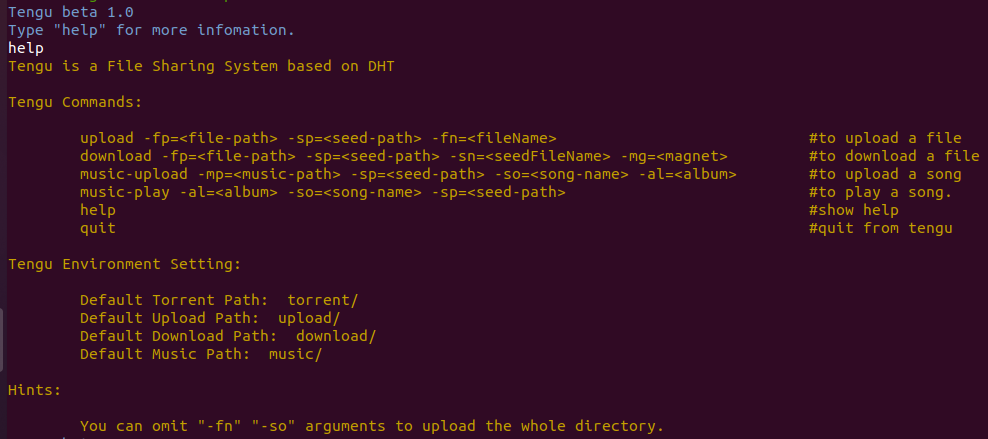
\includegraphics[scale=0.3]{figure/help.png}
\end{figure}

\end{frame}

\begin{frame}{BitTorrent}
\alert{BitTorrent协议}, 一种基于 \alert{TCP/IP} 协议的 P2P 文件传输协议

上传者生成一个 \alert{种子(.torrent)} \\
拿到种子便可以之为索引去 \alert{下载} \\

\\[20pt]

d8:announce0:4:infod6:lengthi11804287e4:name24:Melty \\
\_Land\_Nightmare.mp312:piece lengthi1048576e6:pieces \\
480:b42f29a12ce6ebb8c72cefbb4abf7bed774f936194ac820bd3806739...

\end{frame}

\begin{frame}{Demo演示}
\alert{bith:} BitTorrent Info Hash
\begin{figure}
\centering
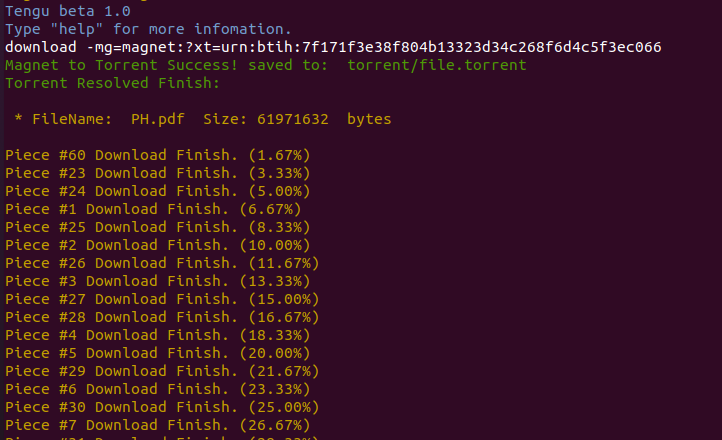
\includegraphics[scale=0.4]{figure/download.png}
\end{figure}
\end{frame}

\begin{frame}{Tengu Music Player}
歌单的存储基于共享文件系统 \\

解析 mp3 格式文件: github.com/faiface/beep \\
\\[20pt]
\begin{figure}
\centering
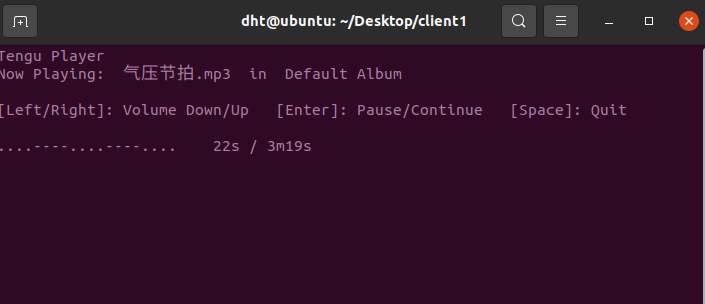
\includegraphics[scale=0.4]{figure/music.png}
\end{figure}

\end{frame}

\section{Reference}

\begin{frame}{Reference}

\begin{itemize}
\item
\alert{dht.pdf} from @xmhuangzhen

\item
\alert{Golang Net} \ (\url{https://pkg.go.dev/net})

\item
\alert{Chord: A Scalable Peer-to-peer Lookup Protocol for Internet Applications}

\item
\alert{Kademlia: A Peer-to-Peer Information System Based on the XOR Metric}

\item
\alert{Building a BitTorrent client from the ground up in Go}

\item
\alert{Kademlia 算法学习} \ (\url{https://shuwoom.com/?p=813})

\end{itemize}

\end{frame}

\begin{frame}[standout]
  \centering
  \textbf{Thank You for Listening!}
\end{frame}

\end{document}